%%%%%%%%%%%%%%%%%%%%%%%%%%%%%%%%%%%%%%%%%
% Lachaise Assignment
% LaTeX Template
% Version 1.0 (26/6/2018)
%
% This template originates from:
% http://www.LaTeXTemplates.com
%
% Authors:
% Marion Lachaise & François Févotte
% Vel (vel@LaTeXTemplates.com)
%
% License:
% CC BY-NC-SA 3.0 (http://creativecommons.org/licenses/by-nc-sa/3.0/)
%
%%%%%%%%%%%%%%%%%%%%%%%%%%%%%%%%%%%%%%%%%

%----------------------------------------------------------------------------------------
%	PACKAGES AND OTHER DOCUMENT CONFIGURATIONS
%----------------------------------------------------------------------------------------

\documentclass{article}

%%%%%%%%%%%%%%%%%%%%%%%%%%%%%%%%%%%%%%%%%
% Lachaise Assignment
% Structure Specification File
% Version 1.0 (26/6/2018)
%
% This template originates from:
% http://www.LaTeXTemplates.com
%
% Authors:
% Marion Lachaise & François Févotte
% Vel (vel@LaTeXTemplates.com)
%
% License:
% CC BY-NC-SA 3.0 (http://creativecommons.org/licenses/by-nc-sa/3.0/)
% 
%%%%%%%%%%%%%%%%%%%%%%%%%%%%%%%%%%%%%%%%%

%----------------------------------------------------------------------------------------
%	PACKAGES AND OTHER DOCUMENT CONFIGURATIONS
%----------------------------------------------------------------------------------------

\usepackage{amsmath,amsfonts,stmaryrd,amssymb} % Math packages

\usepackage{enumerate} % Custom item numbers for enumerations

\usepackage[ruled]{algorithm2e} % Algorithms

\usepackage[framemethod=tikz]{mdframed} % Allows defining custom boxed/framed environments

\usepackage{graphicx} % images

\usepackage{hyperref}
\graphicspath{ {../code/outputs/} }

\usepackage{listings} % File listings, with syntax highlighting
\lstset{
	basicstyle=\ttfamily, % Typeset listings in monospace font
}

%----------------------------------------------------------------------------------------
%	DOCUMENT MARGINS
%----------------------------------------------------------------------------------------

\usepackage{geometry} % Required for adjusting page dimensions and margins

\geometry{
	paper=a4paper, % Paper size, change to letterpaper for US letter size
	top=2.5cm, % Top margin
	bottom=3cm, % Bottom margin
	left=2.5cm, % Left margin
	right=2.5cm, % Right margin
	headheight=14pt, % Header height
	footskip=1.5cm, % Space from the bottom margin to the baseline of the footer
	headsep=1.2cm, % Space from the top margin to the baseline of the header
	%showframe, % Uncomment to show how the type block is set on the page
}

%----------------------------------------------------------------------------------------
%	FONTS
%----------------------------------------------------------------------------------------

\usepackage[utf8]{inputenc} % Required for inputting international characters
\usepackage[T1]{fontenc} % Output font encoding for international characters

\usepackage{XCharter} % Use the XCharter fonts

%----------------------------------------------------------------------------------------
%	COMMAND LINE ENVIRONMENT
%----------------------------------------------------------------------------------------

% Usage:
% \begin{commandline}
%	\begin{verbatim}
%		$ ls
%		
%		Applications	Desktop	...
%	\end{verbatim}
% \end{commandline}

\mdfdefinestyle{commandline}{
	leftmargin=10pt,
	rightmargin=10pt,
	innerleftmargin=15pt,
	middlelinecolor=black!50!white,
	middlelinewidth=2pt,
	frametitlerule=false,
	backgroundcolor=black!5!white,
	frametitle={Command Line},
	frametitlefont={\normalfont\sffamily\color{white}\hspace{-1em}},
	frametitlebackgroundcolor=black!50!white,
	nobreak,
}

% Define a custom environment for command-line snapshots
\newenvironment{commandline}{
	\medskip
	\begin{mdframed}[style=commandline]
}{
	\end{mdframed}
	\medskip
}

%----------------------------------------------------------------------------------------
%	FILE CONTENTS ENVIRONMENT
%----------------------------------------------------------------------------------------

% Usage:
% \begin{file}[optional filename, defaults to "File"]
%	File contents, for example, with a listings environment
% \end{file}

\mdfdefinestyle{file}{
	innertopmargin=1.6\baselineskip,
	innerbottommargin=0.8\baselineskip,
	topline=false, bottomline=false,
	leftline=false, rightline=false,
	leftmargin=2cm,
	rightmargin=2cm,
	singleextra={%
		\draw[fill=black!10!white](P)++(0,-1.2em)rectangle(P-|O);
		\node[anchor=north west]
		at(P-|O){\ttfamily\mdfilename};
		%
		\def\l{3em}
		\draw(O-|P)++(-\l,0)--++(\l,\l)--(P)--(P-|O)--(O)--cycle;
		\draw(O-|P)++(-\l,0)--++(0,\l)--++(\l,0);
	},
	nobreak,
}

% Define a custom environment for file contents
\newenvironment{file}[1][File]{ % Set the default filename to "File"
	\medskip
	\newcommand{\mdfilename}{#1}
	\begin{mdframed}[style=file]
}{
	\end{mdframed}
	\medskip
}

%----------------------------------------------------------------------------------------
%	NUMBERED QUESTIONS ENVIRONMENT
%----------------------------------------------------------------------------------------

% Usage:
% \begin{question}[optional title]
%	Question contents
% \end{question}

\mdfdefinestyle{question}{
	innertopmargin=1.2\baselineskip,
	innerbottommargin=0.8\baselineskip,
	roundcorner=5pt,
	nobreak,
	singleextra={%
		\draw(P-|O)node[xshift=1em,anchor=west,fill=white,draw,rounded corners=5pt]{%
		Question \theQuestion\questionTitle};
	},
}

\newcounter{Question} % Stores the current question number that gets iterated with each new question

% Define a custom environment for numbered questions
\newenvironment{question}[1][\unskip]{
	\bigskip
	\stepcounter{Question}
	\newcommand{\questionTitle}{~#1}
	\begin{mdframed}[style=question]
}{
	\end{mdframed}
	\medskip
}

%----------------------------------------------------------------------------------------
%	WARNING TEXT ENVIRONMENT
%----------------------------------------------------------------------------------------

% Usage:
% \begin{warn}[optional title, defaults to "Warning:"]
%	Contents
% \end{warn}

\mdfdefinestyle{warning}{
	topline=false, bottomline=false,
	leftline=false, rightline=false,
	nobreak,
	singleextra={%
		\draw(P-|O)++(-0.5em,0)node(tmp1){};
		\draw(P-|O)++(0.5em,0)node(tmp2){};
		\fill[black,rotate around={45:(P-|O)}](tmp1)rectangle(tmp2);
		\node at(P-|O){\color{white}\scriptsize\bf !};
		\draw[very thick](P-|O)++(0,-1em)--(O);%--(O-|P);
	}
}

% Define a custom environment for warning text
\newenvironment{warn}[1][Warning:]{ % Set the default warning to "Warning:"
	\medskip
	\begin{mdframed}[style=warning]
		\noindent{\textbf{#1}}
}{
	\end{mdframed}
}

%----------------------------------------------------------------------------------------
%	INFORMATION ENVIRONMENT
%----------------------------------------------------------------------------------------

% Usage:
% \begin{info}[optional title, defaults to "Info:"]
% 	contents
% 	\end{info}

\mdfdefinestyle{info}{%
	topline=false, bottomline=false,
	leftline=false, rightline=false,
	nobreak,
	singleextra={%
		\fill[black](P-|O)circle[radius=0.4em];
		\node at(P-|O){\color{white}\scriptsize\bf i};
		\draw[very thick](P-|O)++(0,-0.8em)--(O);%--(O-|P);
	}
}

% Define a custom environment for information
\newenvironment{info}[1][Info:]{ % Set the default title to "Info:"
	\medskip
	\begin{mdframed}[style=info]
		\noindent{\textbf{#1}}
}{
	\end{mdframed}
}
 % Include the file specifying the document structure and custom commands

%----------------------------------------------------------------------------------------
%	ASSIGNMENT INFORMATION
%----------------------------------------------------------------------------------------

\title{COMP9417: Supplementary Exam} % Title of the assignment

\author{z5113817} % Author name and email address

\date{University of New South Wales --- \today} % University, school and/or department name(s) and a date

%----------------------------------------------------------------------------------------

\begin{document}

% \maketitle % Print the title

%----------------------------------------------------------------------------------------
%	Main Contents
%----------------------------------------------------------------------------------------

% All code for this homework set is available \href{https://github.com/william-coulter/COMP9417\_Homework\_2/tree/master}{here}.

% \newpage

\section*{Question 1}

\subsection*{a}

% 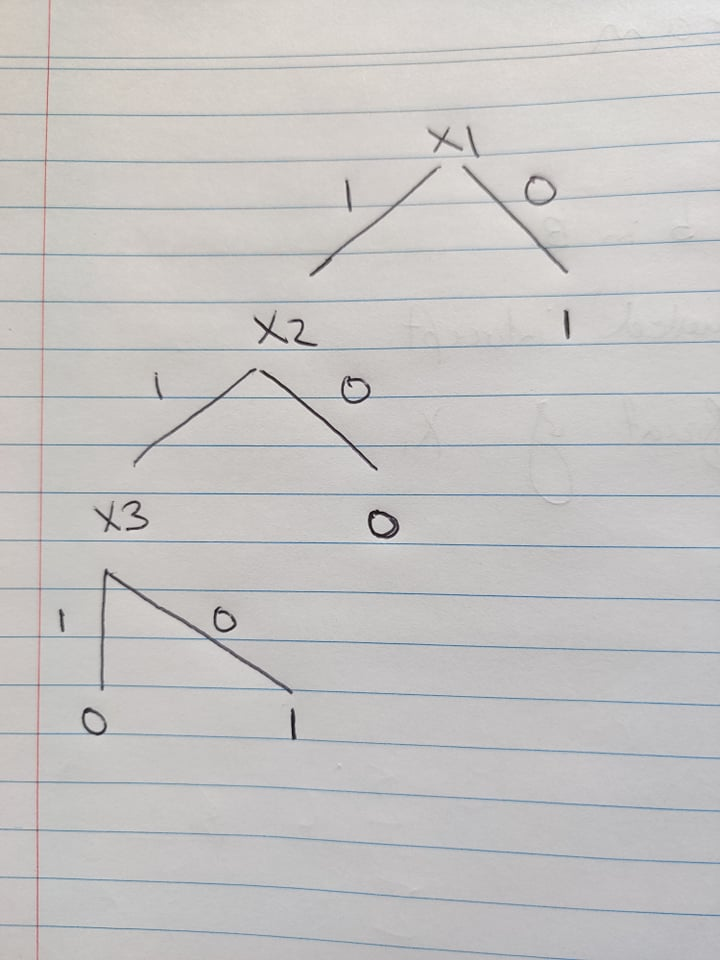
\includegraphics[scale=0.3]{q2a_decision_tree.jpg}

\subsection*{b}

In these regression schemes, \(w_{0}\) acts as the y-intercept of the model and \(w_{1}\) acts as the gradient. Therefore we would expect 
regression scheme (i) to have a larger gradient than (ii) since there is a smaller penalty on \(w_{1}\) (\(\lambda = 1\) vs \(\lambda = 10\) respectively).
Regression schemes (iii) and (iv) would have a smaller y-intercept than (i) and (ii) since \(w_{0}\) is included in their penalties. Scheme (iv) would have 
a smaller gradient and y-intercept than (iii) since its penalty hyperparameter is larger (\(\lambda = 10\)).\\

From the above reasoning, regression scheme (i) matches (a) (it has the largest gradient), (ii) matches (b) (a smaller gradient than (i) but the highest \(w_{0}\) since this
is not in the regression's penalty term), (iii) matches (c) (a relatively small gradient y-intercept) and (iv) matches (d) ((iv) has a large penalty hyperparameter
so the model would be encouraged to have a small gradient and y-intercept. (d) has the smallest y-intercept and a relatively small gradient).

\subsection*{c}

\subsubsection*{i}

The expected error when testing on the training data and \(k = 1\) is 0. Assuming no contradictions in the data, then because the testing data set is 
the same as the training data set and \(k = 1\), there is a classification region for each data point which will correctly classify the original training set.

\subsubsection*{ii}

There are 10,000 data points in total. 50\% of these are positive classes and 50\% are negative classes. In leave-one-out cross validation on 1NN, the data point being considered will be correctly classified if its nearest neighbour 
(but not the data point itself, since we are leaving this out) matches its classification. Even though the distribution classifications varies depending on 
the region of the dataset (e.g. the left rectangle has 25\% +ve and 75\% -ve), each rectangle has the same number of data points so if you are choosing any data point randomly in either rectangular region,
then the probability of that the data point's nearest neighbour matches its classification is 50\%. Therefore the expected error is 5,000.

\subsubsection*{iii}

% Looking at each rectangle, the left rectangle in the test data has no +ve classes whereas in the left rectangle in the training data there are 1,250 (25\%).
% Similarly for the right rectangle in the test data there are no -ve classes but the right rectangle in the the training data has 1,250 (25\%).
Training a 1NN model on the left rectangle of the training data will result in 25\% of the rectangle being a region that classifies a point as +ve class and 
75\% of the rectangle being a region that classifies a point as a -ve class. The left rectangle of the testing data is entirely -ve classes and 
since the data points in the test data are uniformly randomly, each data point has a
75\% chance of landing in a region that classifies the point as negative and therefore correctly. The same is true for the right rectangle region.
So overall, a 1NN model trained on the entire training dataset is expected to correctly classify 75\% of the test data giving it an expected error 
of 2,500.

\subsubsection*{iv}

Looking at the left rectangle of the training data and using 21-NN, you would expect the model to classify the entire region as -ve classes. 
This is because for each point in the left rectangle, of the 21 nearest neighbours, you would expect 25\% to be +ve and 75\% to be -ve so
overall the region is classified as negative. When the training data is used as test data, we know that the 1,250 points that are +ve will 
be incorrectly classified as -ve and therefore the expected error is 1,250. This is the same for the right rectangle however the classifications
are inverted. Overall, you would expect a training set error of 2,500 using a 21-NN classifier model.

\subsection*{d}

\subsubsection*{i}
The space of \(X\) is \(2^{p}\). The space of \(Y\) is 2. Therefore the size of the hypothesis class is \(2^{2^{p}}\).

\subsubsection*{ii}

The probability that the version space is not \(\epsilon-exhausted\) after \(n\) training examples is at most \(|H|e^{-\epsilon n}\).
The number of samples needed to ensure that the sample space has a 0.9 probability (\(P\)) of being \(\epsilon-exhausted\) is:

\[
    n = \frac{1}{\epsilon}(ln|H| + ln(\frac{1}{P}))
\]

Substitute in the values to yield:

\[
    n = \frac{1}{0.1}(ln(2^{2^{10}}) + ln(\frac{1}{0.9}))
\]
\[
    n = 10*(1024*ln(2) + ln(\frac{10}{9}))
\]
\[
    n = 7,098.88
\]

Therefore at least 7,099 data points are needed to ensure the version space is \(\epsilon-exhausted\) with 0.9 probability.

\subsubsection*{iii}

\subsection*{f}



\end{document}
